\chapter{真实世界坐标系下的地图生成与定位方法设计}
\label{cha:chap2}

\section{引言}
\label{sec:2.1}
基于SLAM方法的即时建图和定位方法目前已经发展到的相当成熟,尤其是在无人机、无人车领域,基于视觉SLAM方法进行定位有着积
极地应用,对于实际落地的场景,该系统输出的相机位姿和构建的地图必须具备真实尺度才能够进行导航与定位,此外依靠视觉构建
的地图所处坐标系往往取决于初始化成功后的第一帧多建立的坐标系,这些问题的存在都使得传统SLAM系统难以有实际的使用条件。

对于当前传统的单目视觉SLAM算法,设备简易,处理数据较少,满足实时性的要求,但是也存在只能获取相机坐标系下得到相机位姿
以及无法获取地图实际尺度的问题,无法展开实际应用;对于基于双目视觉的SLAM算法,可以解决地图尺度的问题,但面临成本较高,
相机标定难度大且精度不高,鲁棒性较差等问题;对于融合视觉和IMU传感器的SLAM系统,可以获取真实尺度,以及得到真实世界坐
标系下的相机和地图位姿,但是该系统对于IMU的精度要求较高,且在引入IMU后容易产生累计误差,难以初始化成功等问题。

针对上述问题,本章提出一种融合视觉传感器和二维码标签的单目视觉SLAM方法,在传统SLAM功能的基础上,可以得到相机和地图的
真实尺度,并且根据一定的坐标转换,可以得到真实世界坐标系下的相机位姿和地图。在真实的应用场景中,布置的二维码和普通的自
然关键点相比,更加容易捕捉到关键点,此外,比较固定,在重定位的流程中,往往会有更好的效果。该系统能够具备以下优良特性:
能够对地图进行保存,复用和更新,通过不断完善的先验地图提高系统的鲁棒性;添加二维码信息增强传统SLAM中的重定位问题,此
外通过二维码的尺度在仅适用单目相机的情况下估算出真实地图的尺度;依靠二维码中坐标系和真实世界的坐标系的转化,获取待估计
物体在真实世界下的位姿。
\section{二维码检测与识别方法}
\label{sec:2.2}
\subsection{二维码检测与识别方法}
\label{sec:2.2.1}
二维码和一般的自然关键点相比较,具备比周围环境亮度更低得到的显著特点,如图~\ref{fig:Aruco_Aruco_Gradient}所示;且
二维码本身是一个四边形的区域,可以凭借该特点约束出后续相机的位姿的绝对尺度;并且每一个二维码通过解码都可以获取到一个
独一无二的对应ID号序号,在SLAM重定位的过程中,可以避免高重合区域的误检,在通过视觉检测二维码得到的过程中,我们希望尽
可能多的检出场景中的所有二维码,随后再通过编码对误检值进行剔除。
\begin{figure}[H]
  \centering%
  \subcaptionbox{ArUco二维码原始图像\label{fig:Aruco}}{%    
    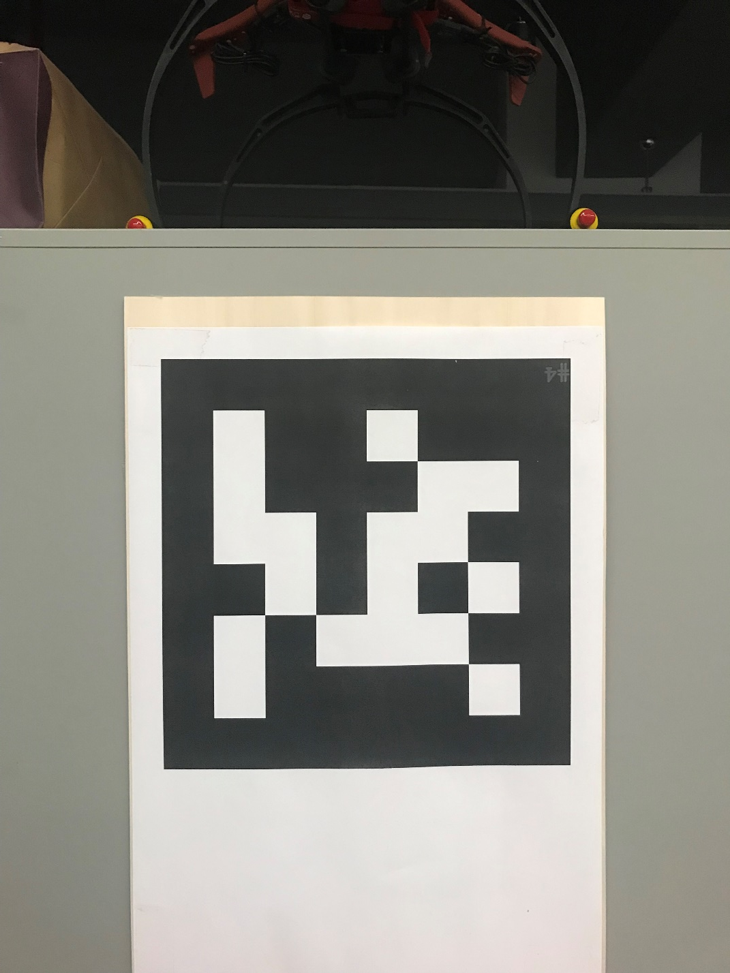
\includegraphics[height=5cm]{Aruco.png}}\hspace{6em}%
  \subcaptionbox{ArUco二维码原始图像\label{fig:Aruco_Gradient}}{%    
    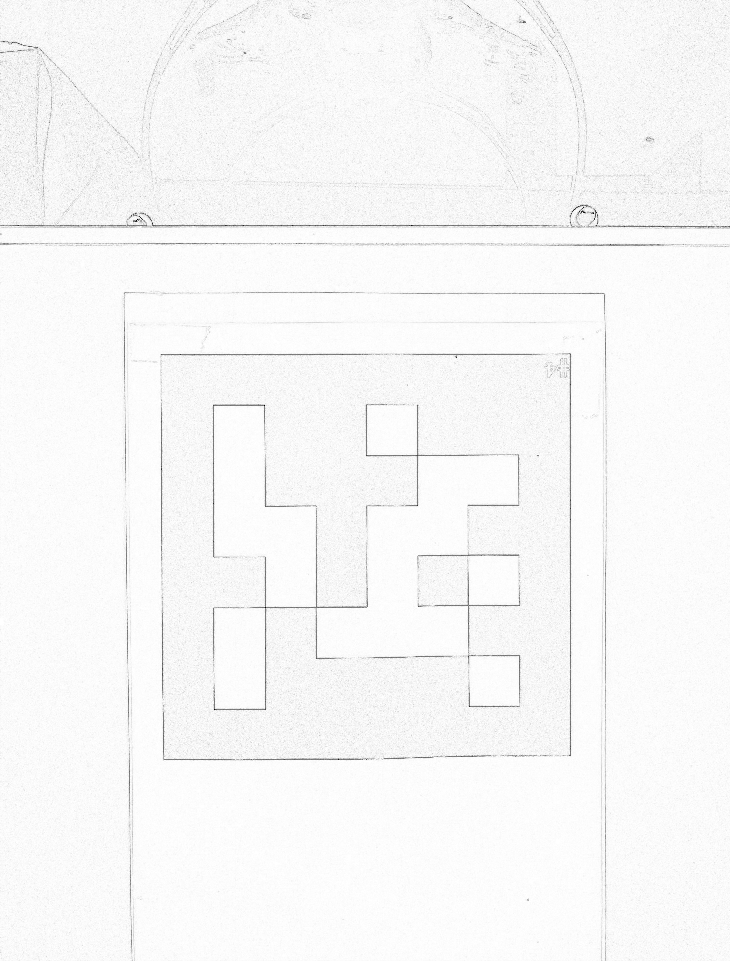
\includegraphics[height=5cm]{Aruco_Gradient.png}}
  \caption{ArUco二维码原始图像和梯度图}
  \label{fig:Aruco_Aruco_Gradient}
\end{figure}

\subsection{ArUco二维码的检测和识别过程}
\label{sec:2.2.2}
ArUco的检测和识别过程主要包括检测出二维码4个角点在图像中的位置,以及被检出的二维码的ID序号,在检测4个角点的位置时,
需要检测图像中的线段和构成二维码的四边形。

在线段检测阶段,首先会计算整个图片中每一个像素的梯度强度大小和方向,随后对计算所得的梯度进行聚类,对所有满足聚类条
件的像素点进行合并,可以的得到一组连续点,即检测出线段。

检测完线段后,进一步的需要检测构成二维码边缘的四边形,针对上一步中获取到的所有线段,对线段进行分组,若满足,上一线
段的末端点和下一线段的起始点之间的距离小于某一阈值,即可首尾进行按照逆时针进行连接,若所有连接的线段数量达到4时,即
认定生成的闭环可能为一个二维码的边缘四边形。

在检测二维码ID值之前,会先设定好一个包含所有二维码的字典,字典的大小即二维码的数量,字典中元素的大小即是每一个二维
码的位数量。检测出构成二维码的四边形后,需要对图像进行透视变化规范图像,随后通过设定阈值分离出二维码上的黑色位和白
色位,通过位数情况即可判断该二维码是否是字典外的不合规值,以及字典中的特定ID值,识别结果如图~\ref{fig:Aruco_detection}
所示。通过这样的方式检测和识别二维码具备非常好的鲁棒性,并且可以对错误值进行效验。
\begin{figure}[H] % use float package if you want it here
  \centering
  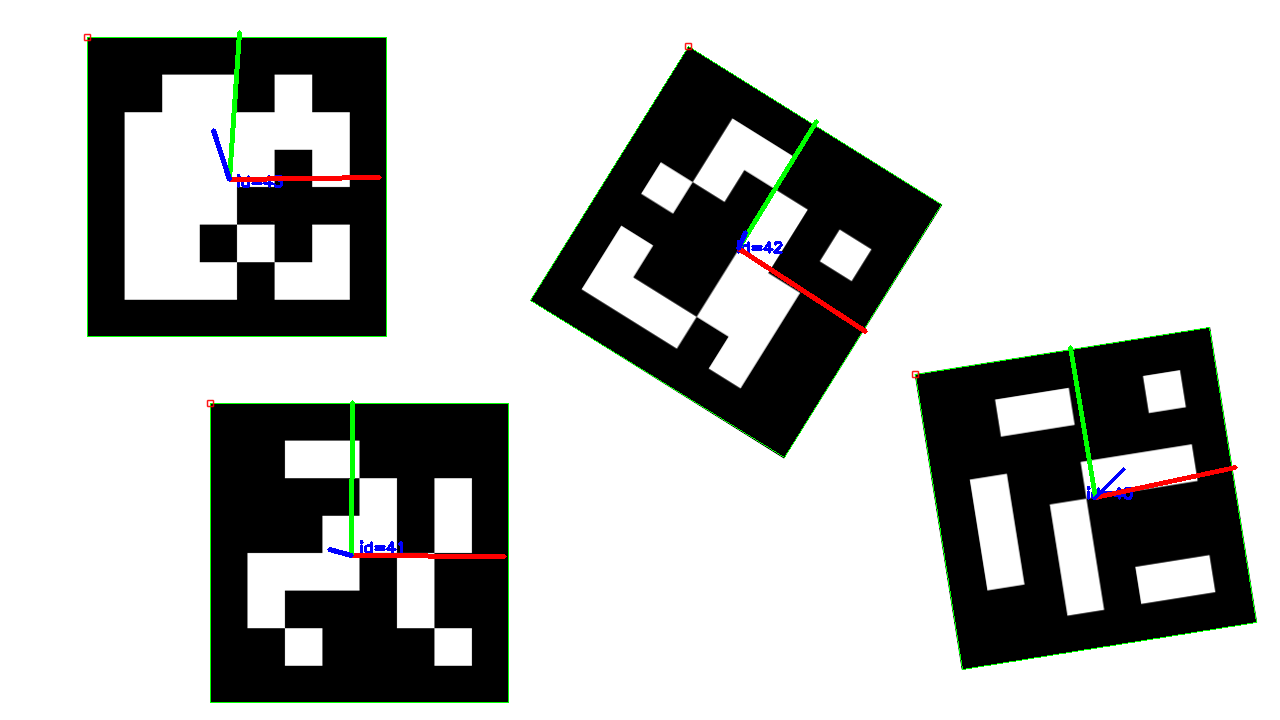
\includegraphics[height=8cm]{Aruco_detection.png}
  \caption{ArUco二维码识别结果示意图}
  \label{fig:Aruco_detection}
\end{figure}

\subsection{估计相机外参}
\label{sec:2.2.3}
对于传入的单帧图像,在提取完二维码的四边形轮廓,4个角点以及检测对应的唯一ID值后,接下来会估计检出的二维码位姿,包括
平移向量和旋转向量,相机的外参主要是通过PnP方法,利用4对点来求解。

为了简化定位的过程,以二维码的坐标系作为世界坐标系,二维码边长为S,则四个角点的坐标分别为A(-S/2,S/2,0),
B(S/2,S/2,0),C(S/2,-S/2,0),D(-S/2,-S/2,0),在图像中的对应像素点为a($u_a$ ,$v_a$),
b($u_b$ ,$v_b$),c($u_c$ ,$v_c$),d($u_d$ ,$v_d$)。因为相机的内参K提前标定,则三维空间中的点和像素坐标中
的点之间的转换关系可以表示为:
\begin{equation}
\begin{split}
  Z{
  \left[ \begin{array}{ccc}
  a\\1
  \end{array} 
  \right ]}=Z{
  \left[ \begin{array}{ccc}
  u_a\\v_a\\1
  \end{array} \right ]}=K{
  \left[ \begin{array}{ccc}
  R&t
  \end{array} \right ]}{
  \left[ \begin{array}{ccc}
  A\\1
  \end{array} \right ]} \\
  ={
  \left[ \begin{array}{ccc}
  f_x & 0 & u_0\\0 & f_y &v_0 \\0 & 0 & 1
  \end{array} \right ]}{
  \left[ \begin{array}{cccc}
  r_{11}&r_{12}&r_{13}&t_1\\r_{21}&r_{7722}&r_{23}&t_2\\r_{31}&r_{32}&r_{33}&t_3
  \end{array} \right ]}{
  \left[ \begin{array}{ccc}
  -s/2\\s/2\\0\\1
  \end{array} \right ]}
\end{split}
\end{equation}

通过以上公式,可以通过二维码到的四个角点求解出相机的旋转矩阵和平移矩阵。
\section{基于二维码的SLAM系统描述}
\label{sec:2.3}
\subsection{包含二维码的地图描述}
\label{sec:2.3.1}
在SLAM运行的过程中,可以生成一套地图系统,对于同一场景,该系统能够复用于后续的建图和定位过程,通过这样得到的方式可以添加对系统
的约束,提高待估计量的精度。传统SLAM系统组成地图的元素主要包括关键点和关键帧,通过对关键点的描述符进行匹配,可以较好的的估计出
相机的位姿。但关键点描述符的计算和匹配过程一般都比较耗时,而且对于重复场景,非常用于出现匹配错误的情况,考虑到这一情况,本文在
此基础上,又添加二维码信息作为构成地图的元素,来进一步优化地图以获取更加准确得到相机位姿。

本文中地图的构成包括以下3个集合:关键点集合p,关键帧集合f和二维码m集合,每个集合之间的数据元素相互耦合关联。关键点集合
\begin{equation}p = \left\{x,v,d\right\}\end{equation}
其中每个元素代表三维空间中的一个点,该点的描述包括在地图坐标系中的三维坐标x,观测方向v以及该点的描述符信息d,考虑到SLAM系统的
实时性,选择BRIEF描述符来加快匹配过程。关键帧集合
\begin{equation}f = \left\{T,K\right\}\end{equation}
其中每一个关键帧包含一个外参矩阵矩阵T(旋转矩阵,平移矩阵),该外参矩阵是全局参考坐标系到相机参考坐标系的转化,K是相机的内参矩阵,
该参数包括相机焦距,光学中心以及畸变参数,这些参数需要在运行SLAM系统之前就准确测量得到。二维码集合
\begin{equation}m = \left\{s,M,x_1,x_2,x_3,x_4\right\}\end{equation}
其中的每一个二维码包括边长s(需要保证场景中的所有二维码的为正方形且所有二维码的尺度完全一致),二维码由其自身坐标系到全局坐标系的
转换矩阵M,$x_1$,$x_2$,$x_3$,$x_4$分别代表二维码四个角点在其自身坐标系下的坐标位置。通过对包含二维码的自然场景进行离线建图,所得地图
如图~\ref{fig:Ucoslam_map}所示,其中正方形代表检出的二维码,蓝色矩形代表检出关键帧,红色点代表检出关键点。
\begin{figure}[H] % use float package if you want it here
  \centering
  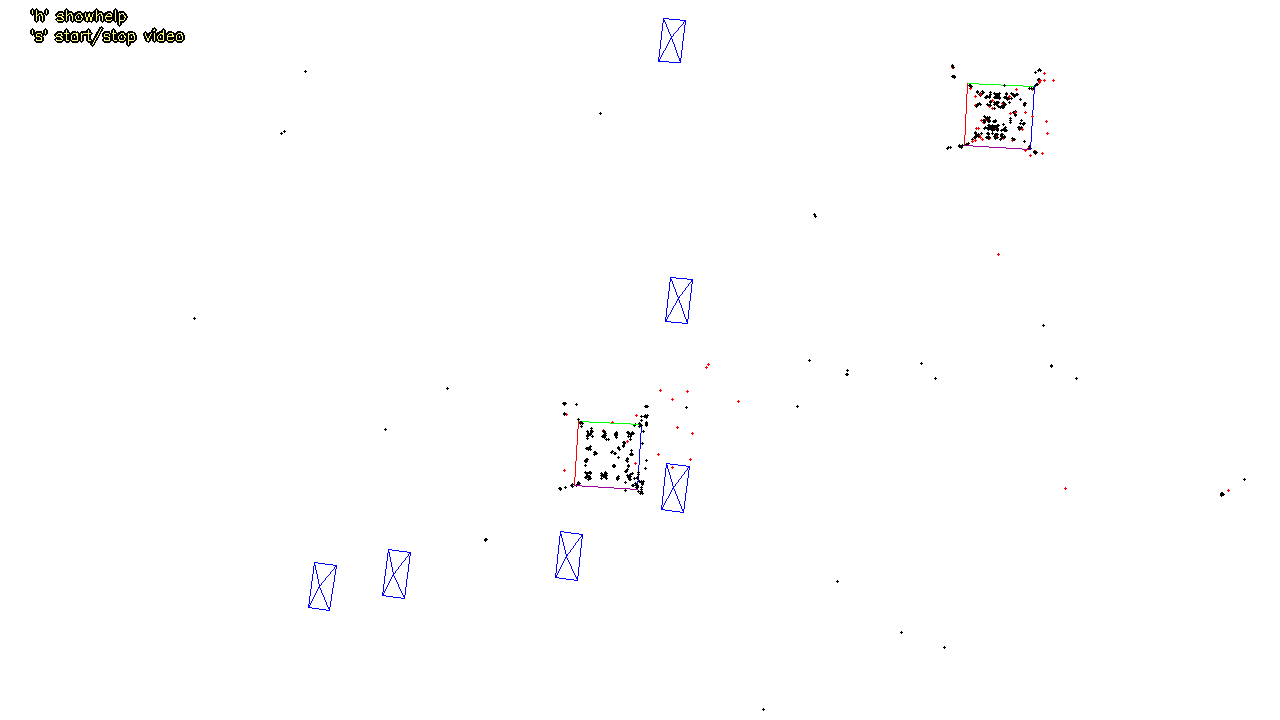
\includegraphics[height=8cm]{Ucoslam_map.png}
  \caption{基于SLAM算法生成的地图}
  \label{fig:Ucoslam_map}
\end{figure}

其中每一类地图元素之间还具备一定的耦合关系,1)对于任意一个关键点,除了自身的属性外,还包括被观测帧序列,即所有可以观测到该特
征点的关键帧的集合,以及在这些帧中出现的像素坐标位置。2)对于任意一个关键帧,还包与其关联的其他关键帧序列,以及在该关键帧中所
有观测到的关键点和坐标。通过这些约束可以使得估计结果有更好的鲁棒性。

\subsection{基于二维码的SLAM过程描述}
\label{sec:2.3.2}
本文所提出的基于二维码的SLAM系统运行流程如图~\ref{fig:slam_pipeline}所示,与一般常见SLAM系统相比较,本文主要提出了结合关键点和二维码标记进行结合
使用。本方法中会一直对地图进行维护,有新的信息加入时,则会对地图进行不断的更新。在对某一个自然场景运行SLAM时,该地图为空,所
以需要对其进行初始化的工作。

当地图初始化完成后,系统进行跟踪和重定位的环节,如果估算出来的相机位姿在某一帧被确定,那么系统会将该帧作为起始帧来估计的位置。
对于跟踪环节,是依靠联合优化关键点和二维码角点的重投影误差进行的。地图的关键帧在系统跟踪前就被选定,并在整个系统中都起着很重
要的作用。
\begin{figure}[H] % use float package if you want it here
  \centering
  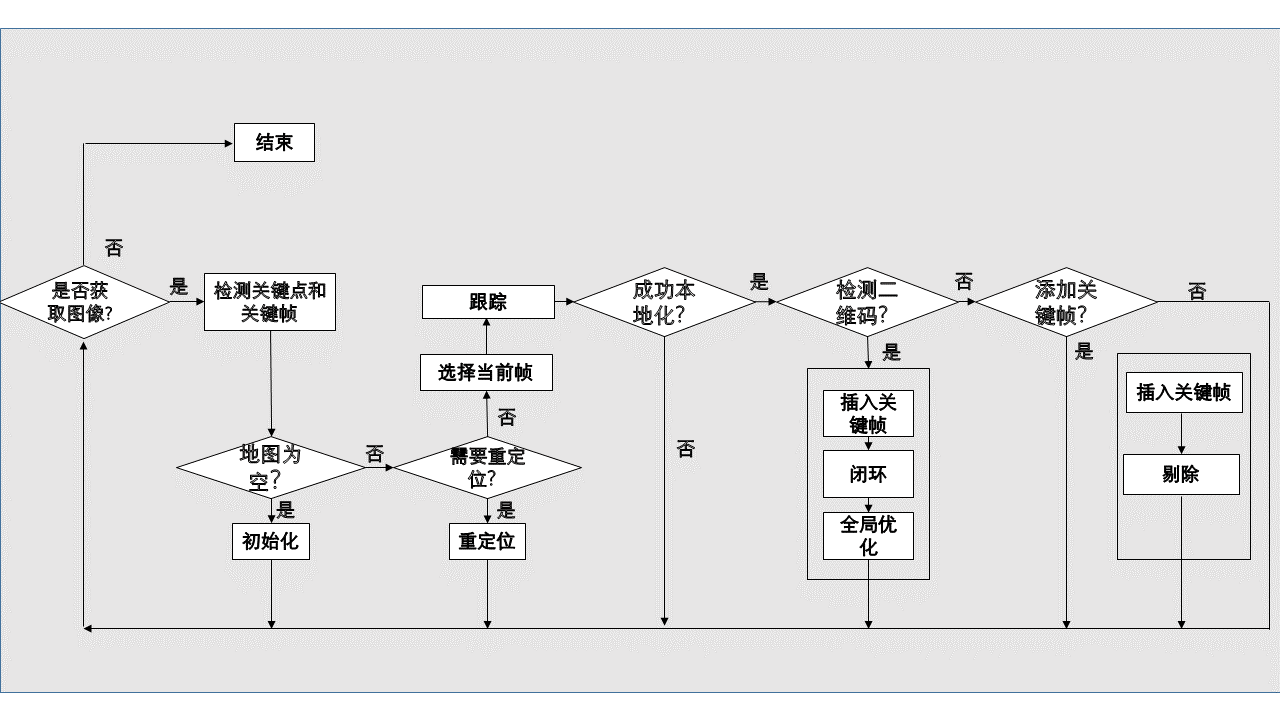
\includegraphics[height=9.5cm]{slam_pipeline.png}
  \caption{基于SLAM算法生成的地图}
  \label{fig:slam_pipeline}
\end{figure}

跟踪成功后,SLAM系统会通过二维码来查询闭环,和单纯基于关键点的闭环检测相比较,二维码的检测必须提前执行,以防止在没有漂移校正
的情况下使用二维码进行跟踪。如果成功检测到闭环,地图的两边需要进行适当的融合,随后将当前帧作为关键帧插入到地图中,并对整个地
图进行全局的优化矫正,提出地图中冗余的信息,保证地图的内存大小维持在一个可以维护的程度。

随后,SLAM系统通过检测关键点来判断是否有闭环出现,若没有检测到,将利用局部优化来整合新的信息,若检测到,则进行全局优化。

如果SLAM系统在跟踪的过程中失效,则进入重定位模式,重定位模式即首先查找地图中已经存在的二维码标记,若找到二维码,则则可以通过
二维码的位置估计出相机的位姿,并通过地图信息进行进一步细化,重新估计相机位姿。若没有找到可见的二维码标记,则在通过传统的BoW方
法来进行重定位。在闭环检测中,将当前帧的关键帧和所有地图中的关键帧进行匹配,并采用RANSAC方法过滤误匹配。如果匹配的成功数量足
够高,则认定重定位成功,并重新进入跟踪模式。


\begin{equation}
\label{equ:chap2:bayes}
p(y|\mathbf{x}) = \frac{p(\mathbf{x},y)}{p(\mathbf{x})}=
\frac{p(\mathbf{x}|y)p(y)}{p(\mathbf{x})}
\end{equation}

\subsection{绘图}
\label{sec:draw}


